\clearpage
\subsection{Signal Uncertainties}
\label{subsec:sig_uncer}


\subsubsection{Scales and PDF uncertainties}
\label{subsec:sig_uncer_scales_PDF}

Additional systematic, as summarized below, are introduced due to modelling differences between various signal Monte Carlo generators.

\begin{itemize}
        \item QCD scale uncertainties (for signal samples generated at NLO QCD);
        \item PDF uncertainty;
\end{itemize}

Those uncertainties on the signal acceptance are included in the fit. They are studied by using truth weight information stored in the current analysis framework flow.

%Some additional scale uncertainties are available in our signal samples; in particular, they refer to some dynamic scale uncertainty obtained by changing the definition of the $\mu_0$. The three available choices:
%
%     \begin{itemize}
%        \item dyn\_scale\_choice\_HT
%        \item dyn\_scale\_choice\_sqrts
%        \item dyn\_scale\_choice\_sum\_pt
%    \end{itemize}

%are combined with the default uncertainties about the variation of the $\mu_f$. This choice has been made consistent with the strategy used here in \cite{Bittrich:2770539}; further information is also provided on the reference.

In particular, for the scale uncertainty we use the envelope of the usual 7 variations as for the background samples and described in Section \ref{subsec:scale_pdf_unc}.

Examples of these uncertaintiy are given in Figures \ref{fig:SigTheoUnc2Lep}-\ref{fig:ScaleUnc1Lep_sig}-\ref{fig:PDFUnc1Lep_sig}-\ref{fig:SigTheoUnc0Lep}.

%2lep
\begin{figure}[ht]
        \centering
    	\subfigure[qcd scale: Merged HP SR]{\includegraphics[width=0.32\textwidth]{figures/2lep/RNN/QCDScale/EW6llqq_0ptag1pfat0pjet_0ptv_SRVBS_HP_RNNScoreMerged_SysTheoryQCD_VBS__1up_Norm.pdf}}
        \subfigure[qcd scale: Merged LP SR]{\includegraphics[width=0.32\textwidth]{figures/2lep/RNN/QCDScale/EW6llqq_0ptag1pfat0pjet_0ptv_SRVBS_LP_RNNScoreMerged_SysTheoryQCD_VBS__1up_Norm.pdf}}
    	\subfigure[qcd scale: resolved SR]{\includegraphics[width=0.32\textwidth]{figures/2lep/RNN/QCDScale/EW6llqq_0ptag2pjet_0ptv_SRVBS_Fid_RNNScoreResolved_SysTheoryQCD_VBS__1up_Norm.pdf}}\\
    	\subfigure[pdf: Merged HP SR]{\includegraphics[width=0.32\textwidth]{figures/2lep/RNN/NNPDF/EW6llqq_0ptag1pfat0pjet_0ptv_SRVBS_HP_RNNScoreMerged_SysTheoryPDF_NNPDF_VBS__1up_Norm.pdf}}
        \subfigure[pdf: Merged LP SR]{\includegraphics[width=0.32\textwidth]{figures/2lep/RNN/NNPDF/EW6llqq_0ptag1pfat0pjet_0ptv_SRVBS_LP_RNNScoreMerged_SysTheoryPDF_NNPDF_VBS__1up_Norm.pdf}}
    	\subfigure[pdf: resolved SR]{\includegraphics[width=0.32\textwidth]{figures/2lep/RNN/NNPDF/EW6llqq_0ptag2pjet_0ptv_SRVBS_Fid_RNNScoreResolved_SysTheoryPDF_NNPDF_VBS__1up_Norm.pdf}}\\
        \caption{QCD scale and PDF uncertainties of the signal MC sample in the 2-lepton channel. Histograms are normalized.}
    \label{fig:SigTheoUnc2Lep}
\end{figure}

%1lep
\begin{figure}[ht]
    \centering
        %\subfigure[Wjets samples, resolved SR]{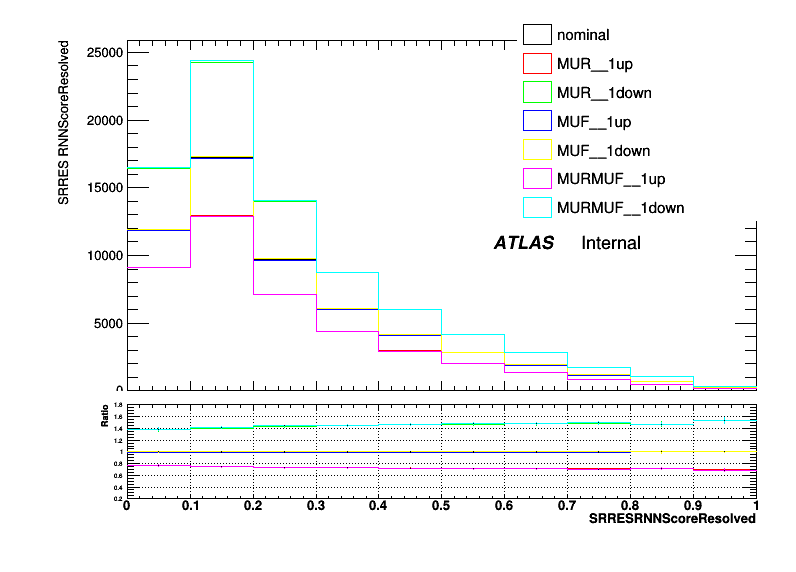
\includegraphics[width=0.3\textwidth]{figures/1lep/PDFUnc/PDFUncWSRRESRNNScoreResolved.png}}
        %\subfigure[Wjets samples, merged HP SR]{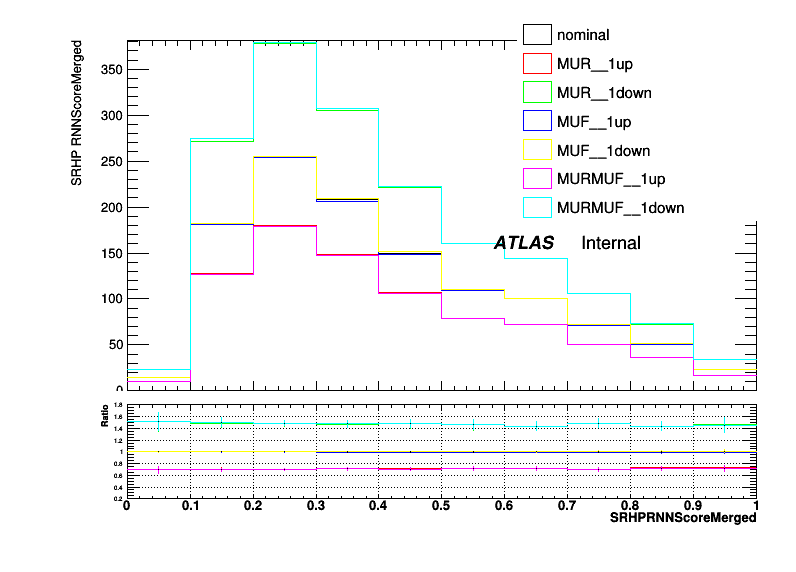
\includegraphics[width=0.3\textwidth]{figures/1lep/PDFUnc/PDFUncWSRHPRNNScoreMerged.png}}
	%\subfigure[Wjets samples, merged LP SR]{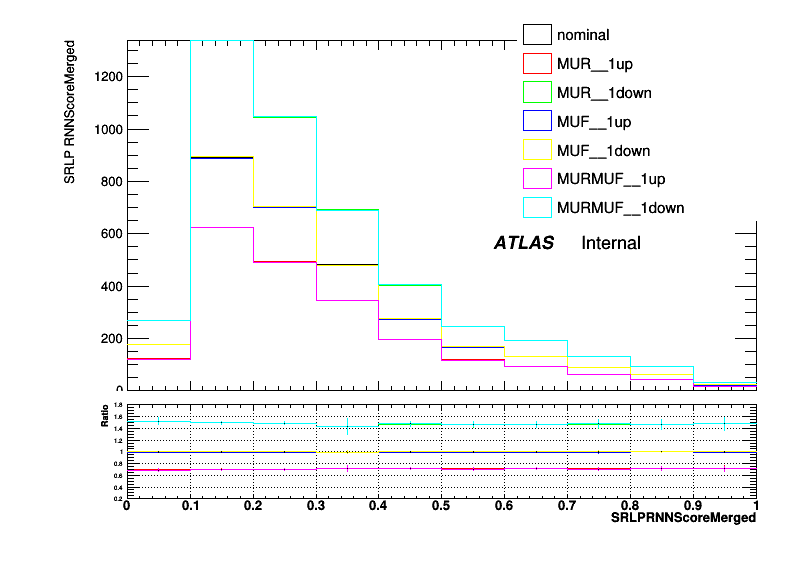
\includegraphics[width=0.3\textwidth]{figures/1lep/PDFUnc/PDFUncWSRLPRNNScoreMerged.png}}\\
        %\subfigure[ttbar samples, resolved SR]{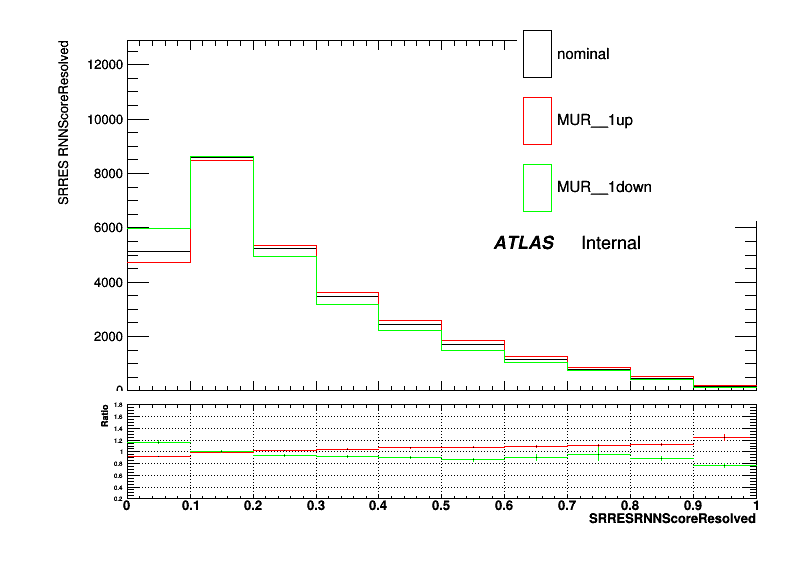
\includegraphics[width=0.3\textwidth]{figures/1lep/PDFUnc/PDFUncttbarSRRESRNNScoreResolved.png}}
        %\subfigure[ttbar samples, merged HP SR]{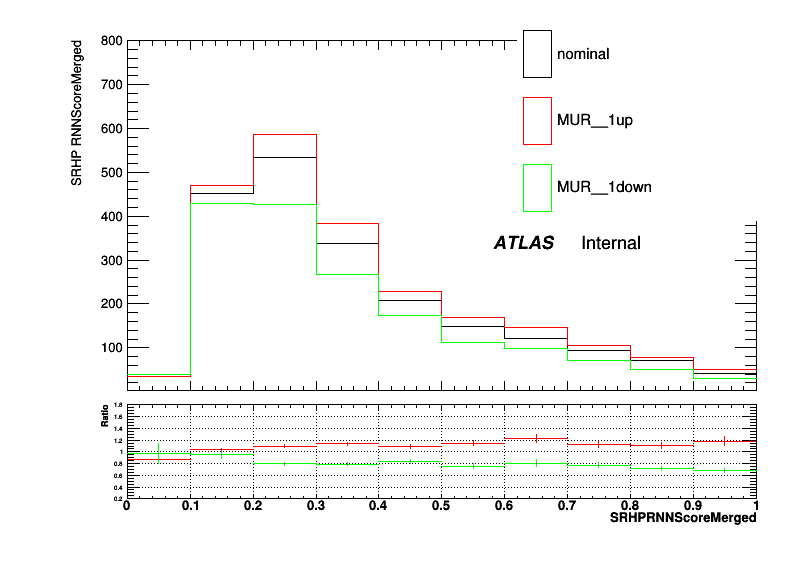
\includegraphics[width=0.3\textwidth]{figures/1lep/PDFUnc/PDFUncttbarSRHPRNNScoreMerged.png}}
	%\subfigure[ttbar samples, merged LP SR]{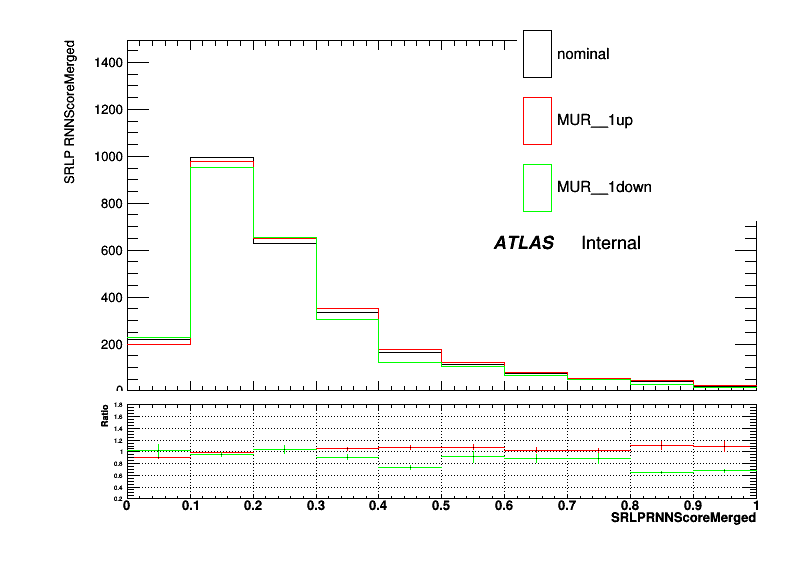
\includegraphics[width=0.3\textwidth]{figures/1lep/PDFUnc/PDFUncttbarSRLPRNNScoreMerged.png}}\\
        \subfigure[signal samples, resolved SR]{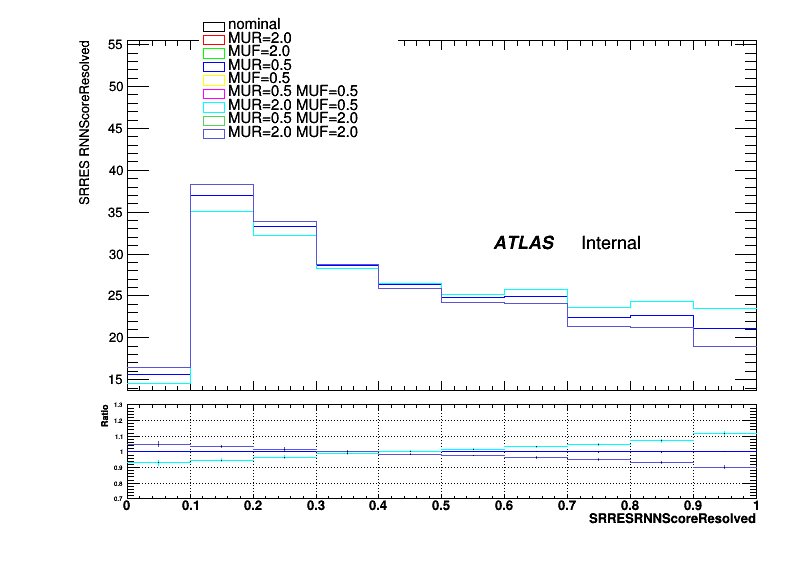
\includegraphics[width=0.3\textwidth]{figures/1lep/PDFUnc/PDFUncEW6SRRESRNNScoreResolved.png}}
        \subfigure[signal samples, merged HP SR]{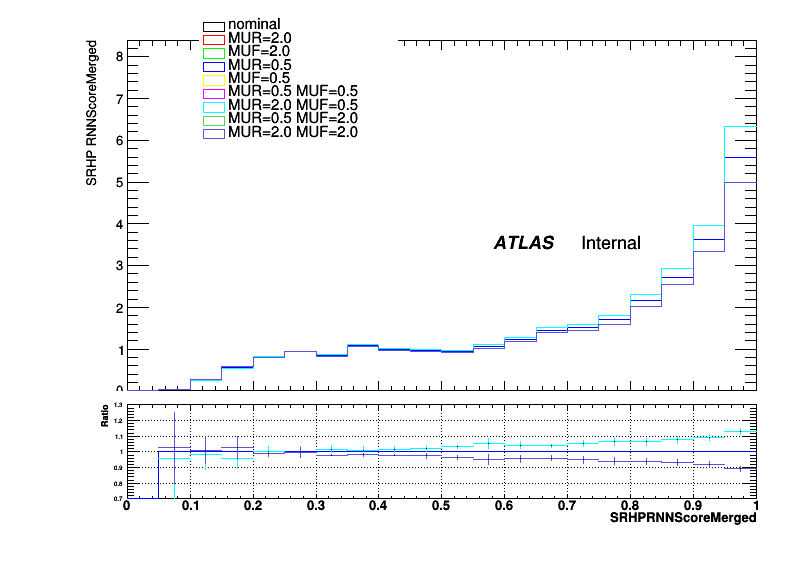
\includegraphics[width=0.3\textwidth]{figures/1lep/PDFUnc/PDFUncEW6SRHPRNNScoreMerged.png}}
	\subfigure[signal samples, merged LP SR]{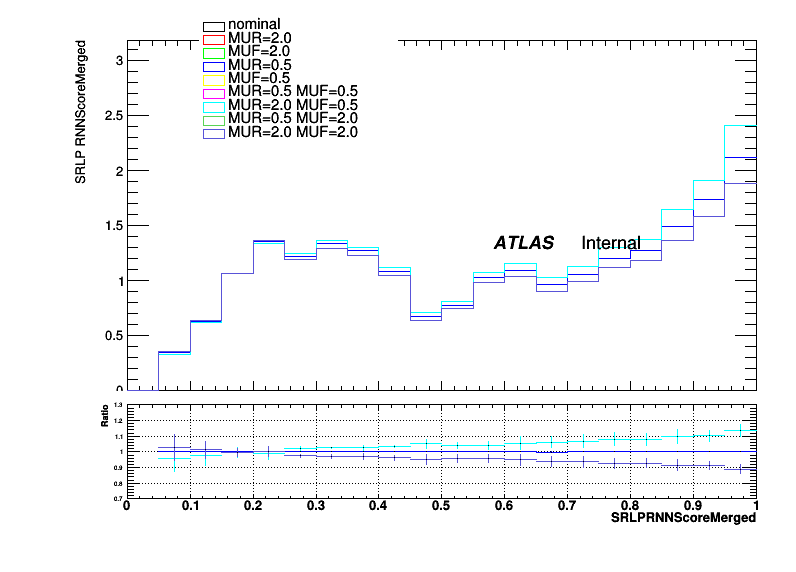
\includegraphics[width=0.3\textwidth]{figures/1lep/PDFUnc/PDFUncEW6SRLPRNNScoreMerged.png}}
        \caption{Scale/Matrix uncertainties for 
%Wjets, ttbar, and 
signal samples in the signal regions, for the 1 lepton channel. Only events from MC16A campaign are shown here. Distributions are not normalized.}
    \label{fig:ScaleUnc1Lep_sig}
\end{figure}

\begin{figure}[ht]
    \centering
        %\subfigure[Wjets samples, resolved SR]{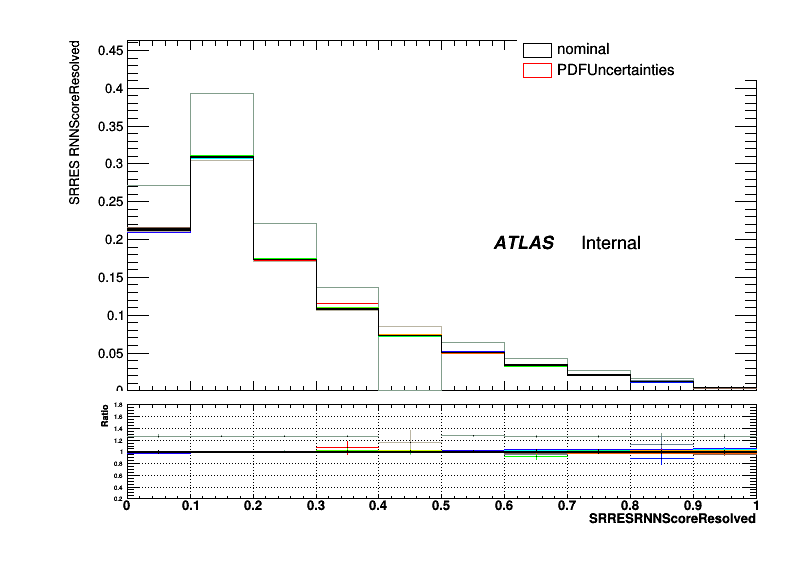
\includegraphics[width=0.3\textwidth]{figures/1lep/PDFUnc/PDFUncWSRRESRNNScoreResolvedPDF.png}}
        %\subfigure[Wjets samples, merged HP SR]{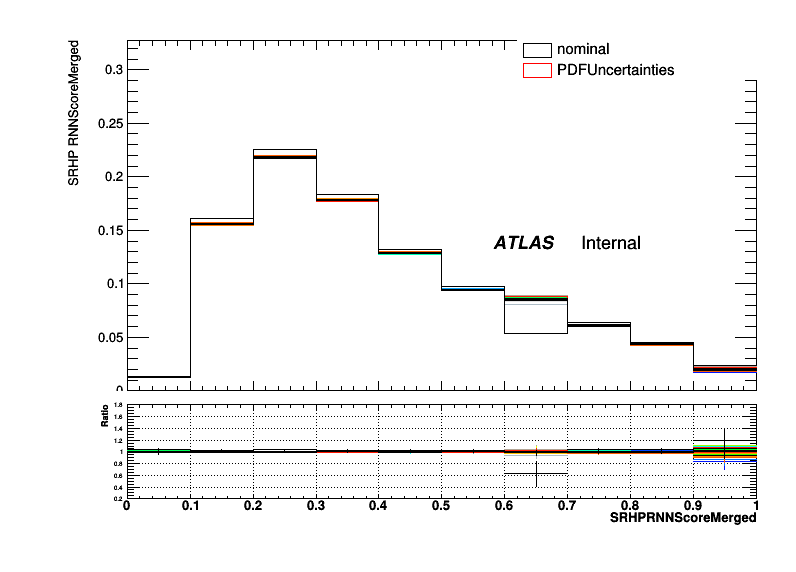
\includegraphics[width=0.3\textwidth]{figures/1lep/PDFUnc/PDFUncWSRHPRNNScoreMergedPDF.png}}
	%\subfigure[Wjets samples, merged LP SR]{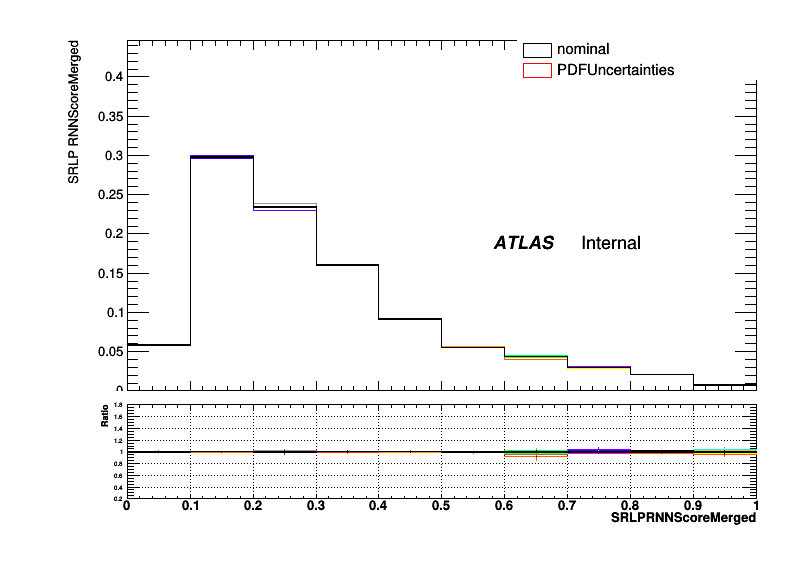
\includegraphics[width=0.3\textwidth]{figures/1lep/PDFUnc/PDFUncWSRLPRNNScoreMergedPDF.png}}\\
        %\subfigure[ttbar samples, resolved SR]{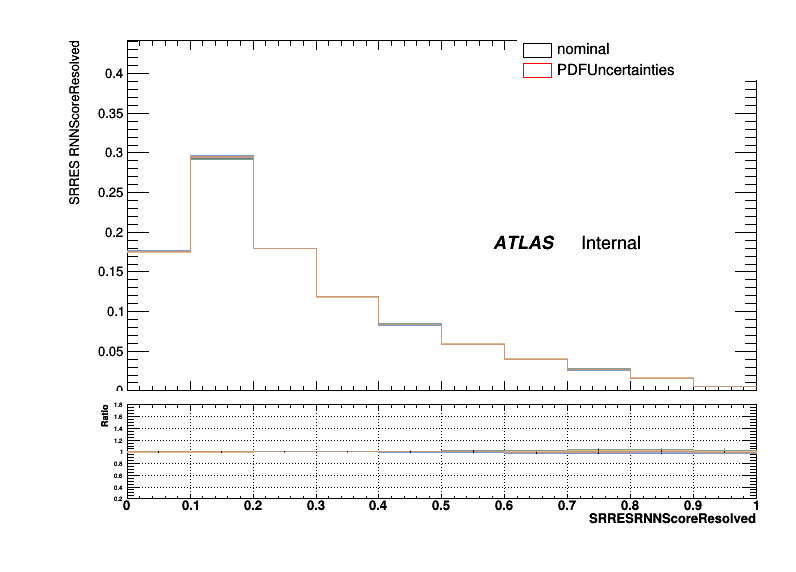
\includegraphics[width=0.3\textwidth]{figures/1lep/PDFUnc/PDFUncttbarSRRESRNNScoreResolvedPDF.png}}
        %\subfigure[ttbar samples, merged HP SR]{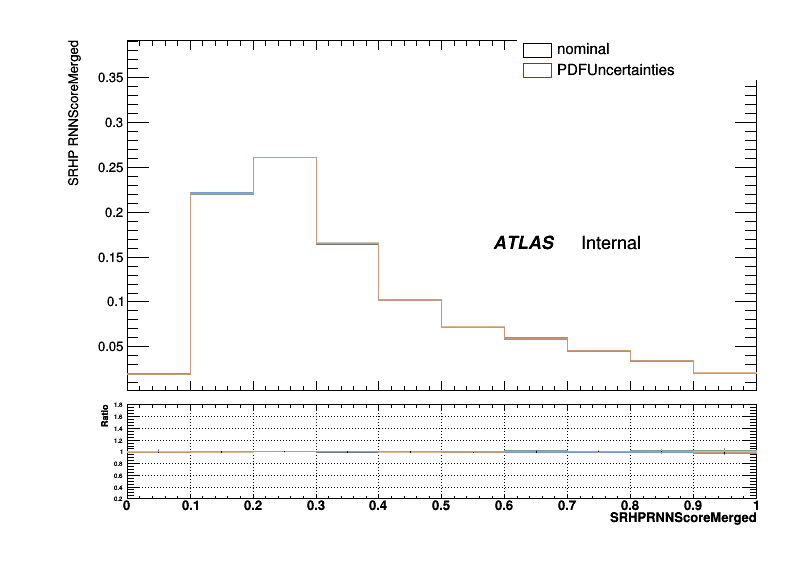
\includegraphics[width=0.3\textwidth]{figures/1lep/PDFUnc/PDFUncttbarSRHPRNNScoreMergedPDF.png}}
	%\subfigure[ttbar samples, merged LP SR]{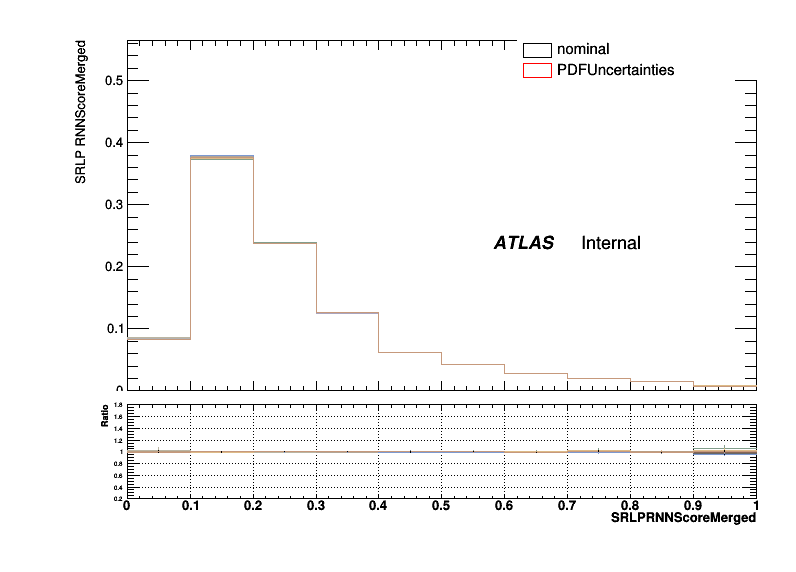
\includegraphics[width=0.3\textwidth]{figures/1lep/PDFUnc/PDFUncttbarSRLPRNNScoreMergedPDF.png}}\\
        \subfigure[signal samples, resolved SR]{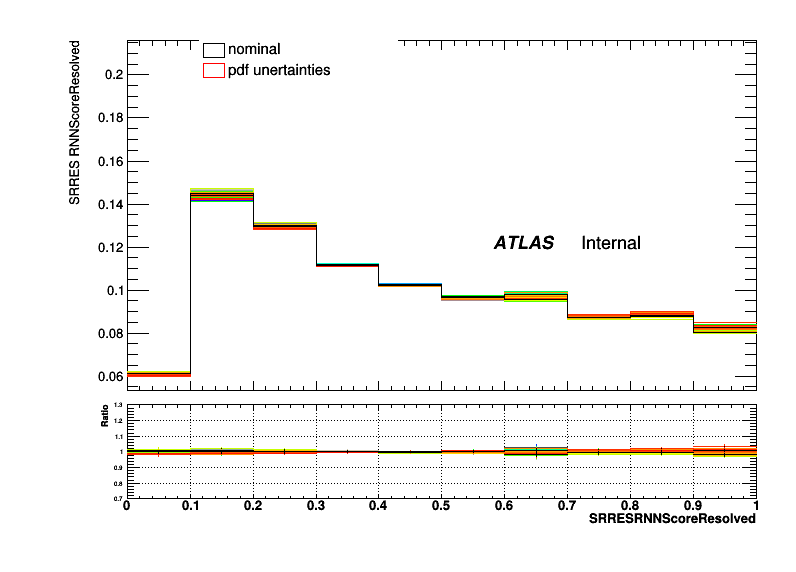
\includegraphics[width=0.3\textwidth]{figures/1lep/PDFUnc/PDFUncEW6SRRESRNNScoreResolvedPDF.png}}
        \subfigure[signal samples, merged HP SR]{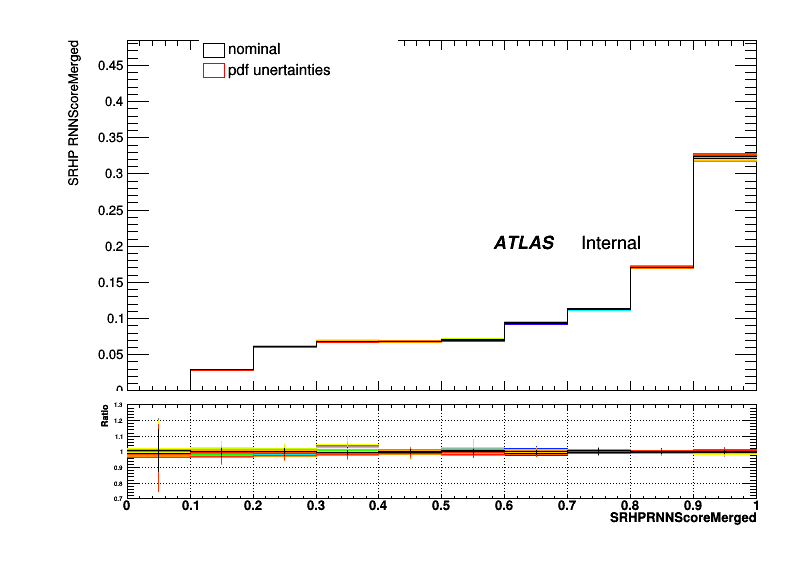
\includegraphics[width=0.3\textwidth]{figures/1lep/PDFUnc/PDFUncEW6SRHPRNNScoreMergedPDF.png}}
	\subfigure[signal samples, merged LP SR]{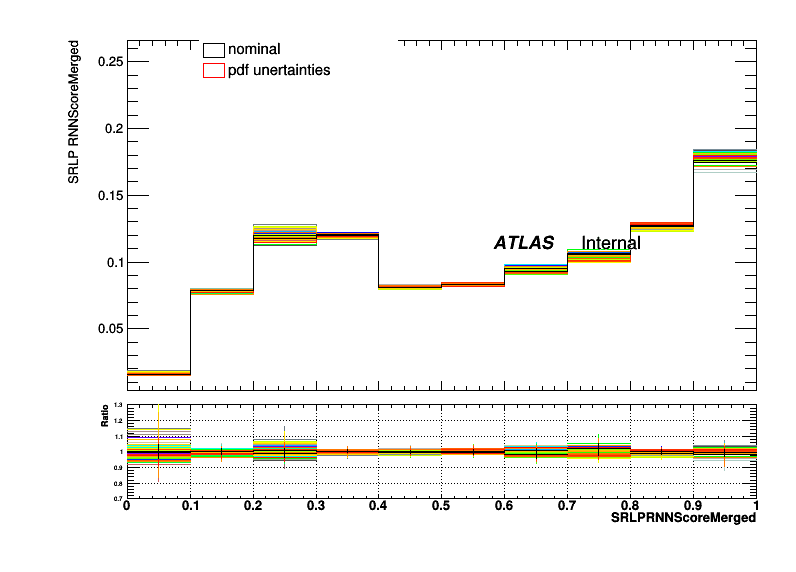
\includegraphics[width=0.3\textwidth]{figures/1lep/PDFUnc/PDFUncEW6SRLPRNNScoreMergedPDF.png}}
        \caption{PDF uncertainties for 
%Wjets, ttbar, and 
signal samples in the signal regions, for the 1 lepton channel. Only events from MC16A campaign are shown here. Distributions are normalized, and pdf variation names are suppressed for clarity. 
%For Wjets samples, a total of 104 pdf variations are shown; for ttbar samples, a total of 43 pdf variations are shown; for signal samples, 
A total of 100 pdf variations are shown. Currently no protection against large weight events were applied, and the rare bin fluctuations are expected to be suppressed with a weight protection in place.}
    \label{fig:PDFUnc1Lep_sig}
\end{figure}

%0lep
\begin{figure}[ht]
        \centering
    	\subfigure[qcd scale: Merged HP SR]{\includegraphics[width=0.32\textwidth]{figures/0lep/systematics/systs/merged/plots/systqcdscaleSigsig_RNN_SRVBS_HP.pdf}}
        \subfigure[qcd scale: Merged LP SR]{\includegraphics[width=0.32\textwidth]{figures/0lep/systematics/systs/merged/plots/systqcdscaleSigsig_RNN_SRVBS_LP.pdf}}
    	\subfigure[qcd scale: resolved SR]{\includegraphics[width=0.32\textwidth]{figures/0lep/systematics/systs/merged/plots/systqcdscaleSigsig_RNN_SRVBS_Fid.pdf}}\\
    	\subfigure[pdf: Merged HP SR]{\includegraphics[width=0.32\textwidth]{figures/0lep/systematics/systs/merged/plots/systinternalpdfSigsig_RNN_SRVBS_HP.pdf}}
        \subfigure[pdf: Merged LP SR]{\includegraphics[width=0.32\textwidth]{figures/0lep/systematics/systs/merged/plots/systinternalpdfSigsig_RNN_SRVBS_LP.pdf}}
    	\subfigure[pdf: resolved SR]{\includegraphics[width=0.32\textwidth]{figures/0lep/systematics/systs/merged/plots/systinternalpdfSigsig_RNN_SRVBS_Fid.pdf}}\\
        \caption{QCD scale and PDF uncertainties of the signal MC sample in the 0-lepton channel}
    \label{fig:SigTheoUnc0Lep}
\end{figure}


\clearpage
\subsubsection{EWK-QCD interference}
\label{subsec:sig_uncer_interf}

As discussed in Section \ref{sec:mc_sample},
EWK and QCD VV+jj samples are generated seprately, therefore, no interference contribution is included.
The actual SM process is, indeed, given by:

\begin{equation}
    \begin{split}
        | M_{SM}(VV+jj) |^2 = | M_{QCD}(VV+jj) + M_{EWK}(VV+jj) |^2 =
                        \\ = |M_{QCD}(VV+jj)|^2 + |M_{EWK}(VV+jj)|^2 + |M_{Int}(VV+jj)|^2
    \end{split}
\end{equation}

In order to estimate the impact of such approximation dedicated (private) samples have been produced
for the inclusive $M_{SM}(VV+jj)$ as well as for the QCD one $M_{QCD}(VV+jj)$; 
this has been done for each of the lepton channel and for the allowed $WW, WZ, ZZ$ boson pairs.

Table \ref{tab:EWKQCDInt_xSec} is summarising the cross section of all the processes according to MG calculation:

\begin{table}[h]
    \centering
    \begin{tabular}{c|c|c|c} 
    \hline 
        Channel              & Inclusive   &  QCD      &    EWK \\    
    \hline 
        ZZ llqq              & $0.2375 \pm 5 \cdot 10^{-4}$  &  $0.2279 \pm 6 \cdot 10^{-4}$    &    $0.00989 \pm 1 \cdot 10^{-5}$\\    
        ZW llqq              & $0.580  \pm 1 \cdot 10^{-3}$  &  $0.536  \pm 1 \cdot 10^{-3}$    &    $0.0461 \pm 1 \cdot 10^{-4}$\\    
        
        WW lvqq              & $209.4 \pm 0.6$    &  $208.4 \pm 0.5$       &    $1.9994 + 1.9777$\\    
        WZ lvqq              & $3.172 \pm 8 \cdot 10^{-3}$  &  $2.921 \pm 6 \cdot 10^{-3}$     &    $0.2600 \pm 6 \cdot 10^{-4}$\\    

        ZZ vvqq              & $0.848 \pm 2 \cdot 10^{-3}$  &  $0.816 \pm 2 \cdot 10^{-3}$     &    $0.03 \pm 8 \cdot 10^{-2}$\\    
        ZW vvqq              & $2.049 \pm 6 \cdot 10^{-3}$  &  $1.892 \pm 4 \cdot 10^{-3}$     &    $0.1572 \pm 5 \cdot 10^{-4}$\\    

    \hline
    \end{tabular}
    \caption{Cross section of the Inclusive, QCD and EWK components of the SM VV+jj production. Note that for WW lvqq sample we rely on baseline EWK samples and the cross sections as reported in Section \ref{sec:mc_sample_ewvvjj}.}
    \label{tab:EWKQCDInt_xSec}
  \end{table}


In this way, an estimation of the interference term can be evaluated as follow:

\begin{equation}
    |M_{Int}(VV+jj)|^2 = | M_{SM}(VV+jj) |^2 - |M_{QCD}(VV+jj)|^2 - |M_{EWK}(VV+jj)|^2
\end{equation}

in particular, since reconstructed level samples are not available for these processes,
we evaluated the impact of such term in the fiducial SRs of the analysis as defined 
in Section \ref{subsec:fidbin_definition}.

Figure \ref{fig:EWKQCDInt_Mjj_0lep}, \ref{fig:EWKQCDInt_Mjj_1lep} and \ref{fig:EWKQCDInt_Mjj_2lep}
show the distribution of the Truth \mjjtag for the \zlep, \olep and \tlep channels 
%l(\textcolor{red}{note: one sample for the \olep channel is currently stucking on the grid, plots will be added later})
.

\begin{figure}[ht]
    \centering
        \subfigure[\zlep - Resolved]{\includegraphics[width=0.45\textwidth]{figures/EWKQCDInt/plot_TagJJM_SR_0lep_Resolved.pdf}}
        \subfigure[\zlep - Merged]{\includegraphics[width=0.45\textwidth]{figures/EWKQCDInt/plot_TagJJM_SR_0lep_Merged.pdf}}
    \caption{Impact of the EWK-QCD interference term on the \mjjtag distribution in \zlep channel for 
                the fiducial Resolved SR (left) and Merged SR (right).}
    \label{fig:EWKQCDInt_Mjj_0lep}
\end{figure}

\begin{figure}[ht]
    \centering
        \subfigure[\olep - Resolved]{\includegraphics[width=0.45\textwidth]{figures/EWKQCDInt/plot_TagJJM_SR_1lep_Resolved.pdf}}
        \subfigure[\olep - Merged]{\includegraphics[width=0.45\textwidth]{figures/EWKQCDInt/plot_TagJJM_SR_1lep_Merged.pdf}}
    \caption{Impact of the EWK-QCD interference term on the \mjjtag distribution in \olep channel for 
                the fiducial Resolved SR (left) and Merged SR (right).}
    \label{fig:EWKQCDInt_Mjj_1lep}
\end{figure}

\begin{figure}[ht]
    \centering
        \subfigure[\tlep - Resolved]{\includegraphics[width=0.45\textwidth]{figures/EWKQCDInt/plot_TagJJM_SR_2lep_Resolved.pdf}}
        \subfigure[\tlep - Merged]{\includegraphics[width=0.45\textwidth]{figures/EWKQCDInt/plot_TagJJM_SR_2lep_Merged.pdf}}
    \caption{Impact of the EWK-QCD interference term on the \mjjtag distribution in \tlep channel for 
                the fiducial Resolved SR (left) and Merged SR (right).}
    \label{fig:EWKQCDInt_Mjj_2lep}
\end{figure}

Since the interference term is found not negligible, a shape uncertainty can be evaluated considering 
the ratio $(EWK+Int) / EWK$ as shown in the ratio pannel of the plots.
In particular, the $max(|R-1|, \Delta R)$ is used as input to build the variations, where R is the ratio
$(EWK+Int) / EWK$ and the $\Delta R$ is the uncertainty on it, as shown in table \ref{tab:IntUnc}.

\begin{landscape}
\begin{table}[h]
    \begin{center} 
    \begin{tabular}{c|c|c|c|c|c|c|c|c|c|c} 
    \hline 
        $(EWK+Int)/EWK$         & & \multicolumn{3}{c|}{\zlep}   & \multicolumn{3}{c|}{ \olep} & \multicolumn{3}{c}{ \tlep} \\    
                                & & R	    &DR	    & max(|R-1|, DR)    & R	    &DR	    & max(|R-1|, DR)    & R	    &DR	    & max(|R-1|, DR) \\
    \hline 
        \multirow{3}{*}{Merged SR}      & 1st bin   & 1,055	& 0,131	& 0,131	& 0,747	& 0,251	& 0,253	& 0,919	& 0,049	& 0,081 \\
                                        & 2nd bin   & 0,956	& 0,096	& 0,096	& 1,122	& 0,184	& 0,184	& 0,999	& 0,041	& 0,041 \\
                                        & 3rd bin   & 0,835	& 0,063	& 0,165	& 1,085	& 0,117	& 0,117	& 0,976	& 0,030	& 0,030 \\
        \multirow{3}{*}{Resolved SR}    & 1st bin   & 0,979	& 0,095	& 0,095	& 1,213	& 0,153	& 0,213	& 0,910	& 0,040	& 0,090 \\
                                        & 2nd bin   & 0,996	& 0,054	& 0,054	& 1,090	& 0,088	& 0,090	& 0,889	& 0,025	& 0,111 \\
                                        & 3rd bin   & 1,012	& 0,034	& 0,034	& 1,091	& 0,054	& 0,091	& 0,924	& 0,018	& 0,076 \\

    \hline
    \end{tabular}
    \caption{Interference uncertainty as a function of the \mjjtag variable for merged and resolved SRs and for each of the lepton channel.}
    \label{tab:IntUnc}
    \end{center} 
  \end{table}
\end{landscape}




The final discriminant model expects the tracks multiplicity of the small-R jets
as input variables and this is a pure reconstruction level information; 
in principle, the tracks multiplicity of the jets is, in first approximation, depending 
only on the $\pt$ and $\eta$ of the jets, so, it could be parametrised in such way
(like performing a DNN or GaussianProcess regression).
To avoid introducing further complexities and to not delay further the timescale of the analysis
we decided to keep the shape parametrisation of the interference term as function of the \mjjtag.
Indeed, this variable is well describing the dependency of the signal phase space
that the final discriminant learnt, as shown in Appendix \ref{app:rnn_2d}.

The final impact of such effect on the shape of the final discriminant at the reconstruction level
SRs is shown in Figure \ref{fig:EWQCDinput_bis}.

\begin{figure}[ht]
    \centering
     \subfigure[Resolved SR]{\includegraphics[width=0.46\textwidth]{figures/EWQCDint/EW6llqq_0ptag2pjet_0ptv_SRVBS_Fid_RNNScoreResolved_SysEWQCDint.pdf}}
     \subfigure[Merged HP SR]{\includegraphics[width=0.46\textwidth]{figures/EWQCDint/EW6llqq_0ptag1pfat0pjet_0ptv_SRVBS_HP_RNNScoreMerged_SysEWQCDint.pdf}}
     \caption{EW-QCD interference systematics uncertainty compared to the nominal distribution, used as input for the fitting.}
     \label{fig:EWQCDinput_bis}
\end{figure}

This uncertainty is used in the final fit model of the analysis 
and the impact of that is documented in Appendix \ref{app:EWQCDint}.



%%% shower uncertainty %%%
\clearpage
\subsubsection{Shower uncertainty}
\label{subsec:sig_uncer_shower}

The impact of the shower on the monte carlo samples generation is included in the final results
as uncertainty on the signal samples.
As mentioned in Section \ref{sec:mc_sample_ewvvjj}, 
dedicated alternative samples have been used for the full set of EWK VV+jj signal samples 
used in the analysis; these samples include Herwig instead of Pythia for the showering effects
and the validation is documented in Appendix \ref{app:H7Gen}.

The impact of the shower effect on both the shape and the normalisation
of the final discriminant is shown in Figures \ref{fig:Shower_SRs}-\ref{fig:Shower_CRs}
for the SRs and CRs respectively.

%%% SRs
\begin{figure}[ht]
    \centering
     \subfigure[\zlep - MergedHP SR]{\includegraphics[width=0.3\textwidth]{figures/ShowerUnc/valid/0lep/SR_HP.pdf}}
     \subfigure[\zlep - MergedLP SR]{\includegraphics[width=0.3\textwidth]{figures/ShowerUnc/valid/0lep/SR_LP.pdf}}
     \subfigure[\zlep - Resolved SR]{\includegraphics[width=0.3\textwidth]{figures/ShowerUnc/valid/0lep/SR_Tight.pdf}} \\
     \subfigure[\olep - MergedHP SR]{\includegraphics[width=0.3\textwidth]{figures/ShowerUnc/valid/1lep/SR_HP.pdf}}
     \subfigure[\olep - MergedLP SR]{\includegraphics[width=0.3\textwidth]{figures/ShowerUnc/valid/1lep/SR_LP.pdf}}
     \subfigure[\olep - Resolved SR]{\includegraphics[width=0.3\textwidth]{figures/ShowerUnc/valid/1lep/SR_Tight.pdf}} \\
     \subfigure[\tlep - MergedHP SR]{\includegraphics[width=0.3\textwidth]{figures/ShowerUnc/valid/2lep/SR_HP.pdf}}
     \subfigure[\tlep - MergedLP SR]{\includegraphics[width=0.3\textwidth]{figures/ShowerUnc/valid/2lep/SR_LP.pdf}}
     \subfigure[\tlep - Resolved SR]{\includegraphics[width=0.3\textwidth]{figures/ShowerUnc/valid/2lep/SR_Tight.pdf}} \\
     \caption{[SRs] Shower systematics uncertainty compared to the nominal distribution, used as input for the fitting.}
     \label{fig:Shower_SRs}
\end{figure}

%%% CRs
\begin{figure}[ht]
    \centering
     \subfigure[\zlep - Merged CR]{\includegraphics[width=0.3\textwidth]{figures/ShowerUnc/valid/0lep/CR_Merged.pdf}}
     \subfigure[\olep - Merged CR]{\includegraphics[width=0.3\textwidth]{figures/ShowerUnc/valid/1lep/CR_Merged.pdf}}
     \subfigure[\tlep - Merged CR]{\includegraphics[width=0.3\textwidth]{figures/ShowerUnc/valid/2lep/CR_Merged.pdf}} \\
     \subfigure[\zlep - Resolved CR]{\includegraphics[width=0.3\textwidth]{figures/ShowerUnc/valid/0lep/CR_Tight.pdf}}
     \subfigure[\olep - Resolved CR]{\includegraphics[width=0.3\textwidth]{figures/ShowerUnc/valid/1lep/CR_Tight.pdf}}
     \subfigure[\tlep - Resolved CR]{\includegraphics[width=0.3\textwidth]{figures/ShowerUnc/valid/2lep/CR_Tight.pdf}} \\
     \subfigure[\olep - MergedHP TopCR]{\includegraphics[width=0.3\textwidth]{figures/ShowerUnc/valid/1lep/CRTop_HP.pdf}}
     \subfigure[\olep - MergedLP TopCR]{\includegraphics[width=0.3\textwidth]{figures/ShowerUnc/valid/1lep/CRTop_LP.pdf}}
     \subfigure[\olep - Resolved TopCR]{\includegraphics[width=0.3\textwidth]{figures/ShowerUnc/valid/1lep/CRTop_Tight.pdf}}
     \caption{[CRs] Shower systematics uncertainty compared to the nominal distribution, used as input for the fitting.}
     \label{fig:Shower_CRs}
\end{figure}
